\documentclass{article}
\usepackage{amsmath}
\usepackage{tikz}

\begin{document}

\begin{center}
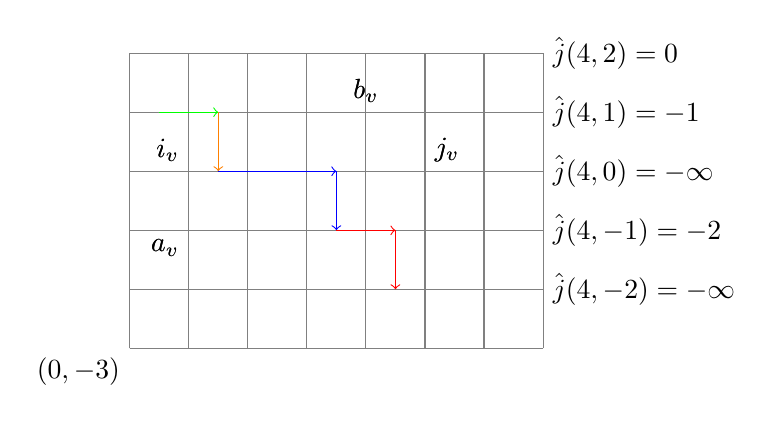
\begin{tikzpicture}[scale=0.75]

% Vertex labels for the left diagram
\node[above left] at (-2, 0) {$i_v$};
\node[below left] at (-2, -1) {$a_v$};
\node[above right] at (2, 0) {$j_v$};
\node[above] at (1, 1) {$b_v$};

% Stochastic six-vertex model configuration for N=2 with packed boundary condition
\draw[step=1cm,gray,thin] (-3,-3) grid (4,2);
\draw[->,green] (-2.5,1) -- (-1.5,1);
\draw[->,orange] (-1.5,1) -- (-1.5,0);
\draw[->,blue] (-1.5,0) -- (0.5,0);
\draw[->,blue] (0.5,0) -- (0.5,-1);
\draw[->,red] (0.5,-1) -- (1.5,-1);
\draw[->,red] (1.5,-1) -- (1.5,-2);

% Boundary conditions for the sample configuration
\node[right] at (4,2) {$\hat{j}(4,2)=0$};
\node[right] at (4,1) {$\hat{j}(4,1)=-1$};
\node[right] at (4,0) {$\hat{j}(4,0)=-\infty$};
\node[right] at (4,-1) {$\hat{j}(4,-1)=-2$};
\node[right] at (4,-2) {$\hat{j}(4,-2)=-\infty$};
\node[below left] at (-3,-3) {$(0,-3)$};

% Labels for the left diagram
\node[above left] at (-2, 0) {$i_v$};
\node[below left] at (-2, -1) {$a_v$};
\node[above right] at (2, 0) {$j_v$};
\node[above] at (1, 1) {$b_v$};

\end{tikzpicture}
\end{center}

\end{document}